\documentclass[12pt, letterpaper]{article}

\usepackage[english]{babel} % Sets the language and regional settings for English documents
\usepackage[utf8]{inputenc} % Allows the use of UTF-8 characters in the document
\usepackage[T1]{fontenc} % Specifies the font encoding
\usepackage[margin=2cm]{geometry} % Sets the page margins
\usepackage{makeidx} % Enables the creation of indexes
\usepackage[numbers]{natbib} % Provides flexible bibliography support
\usepackage{url} % Allows the use of URLs
\usepackage{enumitem} % Customizes the appearance of lists
\usepackage{listings} % Provides syntax highlighting for code listings
\usepackage[dvipsnames]{xcolor} % Allows the use of colors
\usepackage{parskip} % Modifies paragraph spacing
\usepackage{graphicx} % Enables the inclusion of graphics
\usepackage{tikz} % Allows the creation of graphics and diagrams
\usepackage{float}
\usepackage{hyperref} % Enables the creation of hyperlinks
\usepackage{amsmath} % Provides additional math environments and commands
\usepackage{circuitikz} % Allows the creation of electrical circuits
\usepackage{adjustbox} % Adjusts the size of the circuit diagrams
\usepackage{arydshln} % Allows the use of dashed lines in tables
\usepackage{tcolorbox}
\hypersetup{
    colorlinks=true,
    linkcolor=blue,
    urlcolor=blue
}
\usepackage{breakurl} % permite que los links se rompan en varias líneas

\usetikzlibrary{shapes.geometric, positioning}

\lstset{
	language=SQL,
	basicstyle=\ttfamily\small,
	keywordstyle=\color{blue},
	commentstyle=\color[rgb]{0,0.5,0},
	stringstyle=\color{red},
	numbers=left,
	numberstyle=\tiny\color{gray},
	stepnumber=1,
	numbersep=10pt,
	backgroundcolor=\color{white},
	showspaces=false,
	showstringspaces=false,
	breaklines=true,
	frame=single,
	tabsize=2, captionpos=b, lineskip=-1pt,
	extendedchars=true,
	literate={á}{{\'a}}1 {é}{{\'e}}1 {í}{{\'i}}1 {ó}{{\'o}}1 {ú}{{\'u}}1 {Á}{{\'A}}1 {É}{{\'E}}1 {Í}{{\'I}}1 {Ó}{{\'O}}1 {Ú}{{\'U}}1 {ñ}{{\~n}}1 {Ñ}{{\~N}}1 {¿}{{\textquestiondown}}1 {¡}{{\textexclamdown}}1
}

\graphicspath{ {./img/} } % Sets the path for the graphics

\newlist{biblio}{enumerate}{1}
\setlist[biblio,1]{label=[\arabic*]}

\makeindex

\begin{document}

\begin{titlepage}

	\begin{tikzpicture}[remember picture,overlay]
		\node[anchor=north west, inner sep=30] at (current page.north west) {
			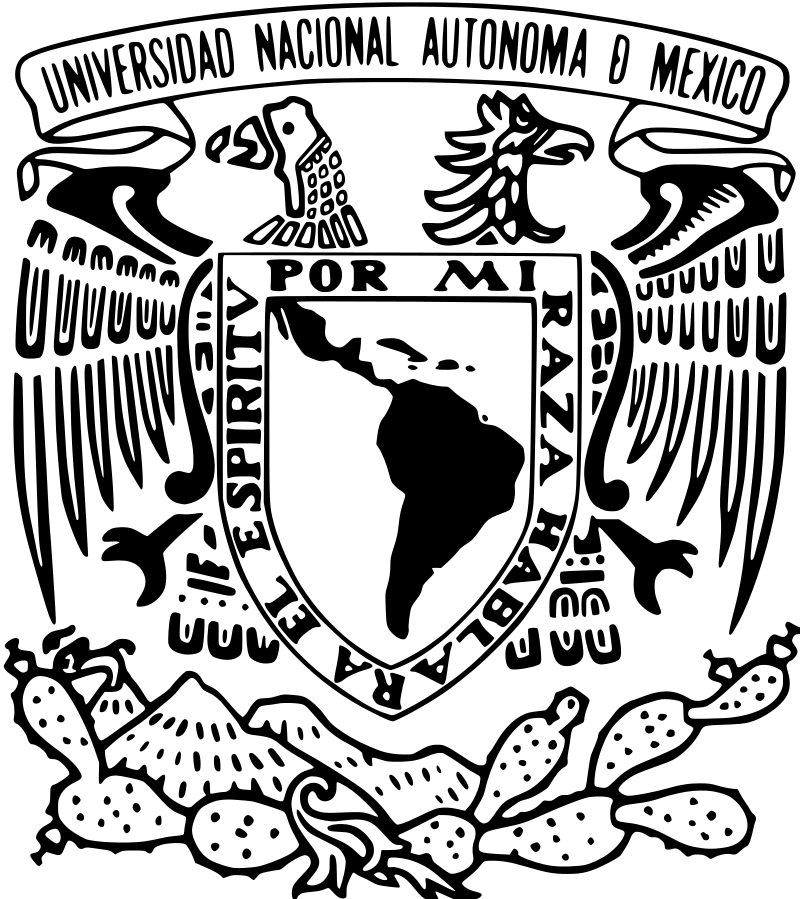
\includegraphics[width=4cm]{escudoUNAM.png}
		};

		\node[anchor=north east, inner sep=30] at (current page.north east) {
			
\includegraphics[width=4cm]{escudoFI.png}
		};
	\end{tikzpicture}

	\begin{center}
		\vspace*{3cm}

		\Huge
		\textbf{Previo 1 - Sistemas eléctricos de primero y segundo orden}

		\vspace{2.5cm}

		\Huge
		\textbf{Facultad de Ingeniería}\\
		Circuitos Eléctricos\\
		Semestre 2025-2\\

		\vspace{2.5cm}

		\textbf{Grupo Laboratorio: 4} 

		\vspace{2.5cm}

		\Huge
		Ugartechea González Luis Antonio\\
        Tepal Briseño Hansel Yael\\
		\textbf{Fecha de entrega: 19/08/2025 } 
		\vspace{2.5cm}
	\end{center}

\end{titlepage}

\section{Determine la función de transferencia del circuito RL}

\begin{center}
    \begin{circuitikz}[american, dot/.style={circle, inner sep=1.5pt, fill=black}]
        % Source and resistor
        \draw (0,0) 
            to[V, invert, l=$V_{in}(s)$] (0,3)
            to[R, l=$R$, i=$i(t)$] (3,3) -- (4,3)
            (0,0) -- (4,0);

        % Output terminals
        \draw (4,3) -- (5,3) node[dot, label=right:$+$] (pvout) {}
              (4,0) -- (5,0) node[dot, label=right:$-$] (nvout) {};

        % Inductor in parallel with Vout
        \draw (4,3) to[L, l=$L$] (4,0);

        % Vout label
        \path let \p1 = (pvout), \p2 = (nvout) in
            node[right] at ($(\p1)!.5!(\p2)$) {$V_{out}(s)$};
    \end{circuitikz}
\end{center}

De acuerdo a las leyes de Kirchhoff tenemos lo siguiente para obtener el voltaje de salida:

\[V_{in}(s) = V_R(s) + V_L(s) = V_R(s) + V_{out}(s)\]

Donde:
\begin{center}
    \begin{tabular}{|c|c|}
        \hline
        \(V_R(s)\) & \(V_{out}(s)\) \\
        \hline
        \(I(s)Z_R\) & \(I(s)Z_L\) \\
        \hline
    \end{tabular}
\end{center}

Despejando la siguiente expresión:

\[V_{in}(s) = I(s)Z_R + I(s)Z_L\]

tenemos:

\[I(s) = \frac{V_{in}(s)}{Z_R + Z_L}\]

Para obtener \(V_{out}\) utilizando las ley de Ohm tenemos:

\[V_{out}(s) = I(s) \cdot Z_L = V_{in}(s)\cdot \frac{Z_L}{Z_R + Z_L}\]

Sustituyendo las impedancias de Laplace:

\[V_{out}(s) = V_{in}(s) \cdot \frac{sL}{R + sl}\]

Entonces tenemos que la función de transferencia está dado por:

\begin{center}
    \begin{tcolorbox}[colframe=red!80!black, width=8cm, sharp corners]
        \[
        H(s) = \frac{V_{out}(s)}{V_{in}(s)} = \frac{sL}{R + sL}
        \]
    \end{tcolorbox}
\end{center}


\section{A partir del resultado anterior determine la constante del tiempo}

Para determinar la constante del tiempo tenemos que tomar en cuenta cuando el denominador del sistema sea igual a cero es decir:
 
\[R + sL = 0\]

Despejando tenemos:

\[s = - \frac{R}{L}\]

Por definición la constante del tiempo es el inverso del valor absoluto del polo, entonces:

\[\tau = \frac{1}{|s_{polo}|}\]

Sustituyendo:

\[\tau = \frac{1}{|-\frac{R}{L}|} = \frac{L}{R}\]

Por lo tanto la constante del tiempo es:

\begin{center}
    \begin{tcolorbox}[colframe=red!80!black, width=4cm, sharp corners]
        \[
        \tau = \frac{L}{R}
        \]
    \end{tcolorbox}
\end{center}

\section{Determine la función de transferencia del circuito RC}

\begin{center}
    \begin{circuitikz}[american, dot/.style={circle, inner sep=1.5pt, fill=black}]
        % Source and resistor
        \draw (0,0) 
            to[V, invert, l=$V_{in}(s)$] (0,3)
            to[R, l=$R$, i=$i(t)$] (3,3) -- (4,3)
            (0,0) -- (4,0);

        % Output terminals
        \draw (4,3) -- (5,3) node[dot, label=right:$+$] (pvout) {}
              (4,0) -- (5,0) node[dot, label=right:$-$] (nvout) {};

        % Capacitor in parallel with Vout
        \draw (4,3) to[C, l=$C$] (4,0);

        % Vout label
        \path let \p1 = (pvout), \p2 = (nvout) in
            node[right] at ($(\p1)!.5!(\p2)$) {$V_{out}(s)$};
    \end{circuitikz}
\end{center}

De acuerdo a las leyes de Kirchhoff tenemos lo siguiente para obtener el voltaje de salida:

\[
V_{in}(s) = V_R(s) + V_C(s) = V_R(s) + V_{out}(s)
\]

Donde:
\begin{center}
    \begin{tabular}{|c|c|}
        \hline
        \(V_R(s)\) & \(V_{out}(s)\) \\
        \hline
        \(I(s)Z_R\) & \(I(s)Z_C\) \\
        \hline
    \end{tabular}
\end{center}

Despejando la siguiente expresión:

\[
V_{in}(s) = I(s)Z_R + I(s)Z_C
\]

tenemos:

\[
I(s) = \frac{V_{in}(s)}{Z_R + Z_C}
\]

Para obtener \(V_{out}\) utilizando la ley de Ohm tenemos:

\[
V_{out}(s) = I(s) \cdot Z_C = V_{in}(s)\cdot \frac{Z_C}{Z_R + Z_C}
\]

Sustituyendo las impedancias de Laplace:

\[
Z_R = R, \quad Z_C = \frac{1}{sC} \quad \Rightarrow \quad V_{out}(s) = V_{in}(s) \cdot \frac{\frac{1}{sC}}{R + \frac{1}{sC}}
\]

Simplificando:

\[
V_{out}(s) = V_{in}(s) \cdot \frac{1}{1 + sRC}
\]

Entonces tenemos que la función de transferencia está dado por:

\begin{center}
    \begin{tcolorbox}[colframe=red!80!black, width=8cm, sharp corners]
        \[
        H(s) = \frac{V_{out}(s)}{V_{in}(s)} = \frac{1}{1 + sRC}
        \]
    \end{tcolorbox}
\end{center}

\section{A partir del resultado anterior determine la constante del tiempo}

Para determinar la constante del tiempo tenemos que tomar en cuenta cuando el denominador del sistema sea igual a cero es decir:
 
\[
1 + sRC = 0
\]

Despejando tenemos:

\[
s = - \frac{1}{RC}
\]

Por definición la constante del tiempo es el inverso del valor absoluto del polo, entonces:

\[
\tau = \frac{1}{|s_{polo}|}
\]

Sustituyendo:

\[
\tau = \frac{1}{|\,-\frac{1}{RC}\,|} = RC
\]

Por lo tanto la constante del tiempo es:

\begin{center}
    \begin{tcolorbox}[colframe=red!80!black, width=4.5cm, sharp corners]
        \[
        \tau = RC
        \]
    \end{tcolorbox}
\end{center}

\section{Determine la función de transferencia del circuito RLC}

\begin{center}
    \begin{circuitikz}[american, dot/.style={circle, inner sep=1.5pt, fill=black}]
        % Fuente de voltaje
        \draw (0,0) 
            to[V, invert, l=$V_{in}(s)$] (0,4)
            to[R, l=$R$, i=$i(t)$] (3,4) 
            to[L, l=$L$] (6,4) -- (7,4)
            (0,0) -- (7,0);

        % Terminales de salida
        \draw (7,4) -- (8,4) node[dot, label=right:$+$] (pvout) {}
              (7,0) -- (8,0) node[dot, label=right:$-$] (nvout) {};

        % Inductor y capacitor en paralelo con la salida
        \draw (7,4) to[C, l=$C$] (7,0);

        % Etiqueta de Vout
        \path let \p1 = (pvout), \p2 = (nvout) in
            node[right] at ($(\p1)!.5!(\p2)$) {$V_{out}(s)$};
    \end{circuitikz}
\end{center}

Conociendo de Antemano que la función de transferencia es igual a:

\[H(s) = \frac{Y(s)}{X(s)}\]

Por lo que a partir del circuito propuesto es necesario conocer las ecuaciones diferenciales que rigen el comportamiento de cada uno de los componentes que participan para encontrar a \(H(s)\), siendo respectivamente:

\begin{itemize}
    \item En la resistencia:
        \begin{equation}
            V_R = I_R \cdot R
            \label{1}
        \end{equation} 
    \item En el inductor: 
        \begin{equation}
            V_L (t) = L \frac{d(I_L)}{dt}
            \label{2}
        \end{equation}
    \item En el capacitor: 
        \begin{equation}
            I_C = C\frac{d(V_c)}{dt}
            \label{3}
        \end{equation}
\end{itemize}

Una vez conociendo estas ecuaciones aplicamos las leyes de voltaje Kirchhoff en la malla del circuito, obteniendo el siguiente resultado:

\begin{equation}
    V_i - V_R - V_L - V_C = 0
    \label{4}
\end{equation}

Donde:
\begin{itemize}
    \item \(V_i\) es el voltaje de entrada
    \item \(V_R\) es el voltaje en la resistencia
    \item \(V_L\) es el voltaje en el inductor
    \item \(V_C\) es el voltaje en el capacitor, que a su vez es el voltaje de salida.
\end{itemize}
Sustituyendo \eqref{1} y \eqref{2}  en \eqref{4} obtenemos la siguiente ecuación:

\begin{equation}
    V_i = I_R \cdot R + L \frac{d(I_L)}{dt} + V_c
    \label{5}
\end{equation}

Al ser un circuito en serie, la corriente es la misma en cada uno de los elementos de este por lo que al sustituir \eqref{3} en \eqref{5} obtenemos:

\begin{equation}
    Vi = RC\frac{d(V_c)}{dt} + LC \frac{d^2(V_c)}{dt^2} + V_c
    \label{6}
\end{equation}

Obteniendo así un sistema de segundo orden que al aplicar la Transformada de Laplace podemos obtener la siguiente ecuación:

\begin{equation}
    Vi = LC V_cs^2 + RCV_c s + V_c
    \label{7}
\end{equation}

Sacando el factor Común y despejando la ecuación obtenemos: 

\begin{equation}
    \frac{V(c)}{V_i} = \frac{1}{LCs^2 + RCs + 1}
    \label{8}
\end{equation}

Encontrando así nuestra función de transferencia para un circuito RLC.
\begin{center}
        \begin{tcolorbox}[colframe=red!80!black, width=8cm, sharp corners]
            \[H(s) = \frac{1}{LCs^2 + RCs + 1}\]
        \end{tcolorbox}
\end{center}

\section{A partir del resultado anterior exprese \(w_n\) y \(\delta\) en función de R, L y C}

Sabiendo que la función de transferencia de segundo orden tiene la forma:
\begin{equation}
    H(s) = \frac{w_n^2}{s^2 + 2 \delta w_ns + w_n^2}
    \label{9}
\end{equation}

Es necesario normalizar nuestra función de transferencia para poder encontrar los valores de \(w_n\) y \(\delta\), por lo que multiplicaremos \eqref{8} por \(\frac{1}{LC}\) para que se asemeje a \eqref{9}.

\begin{equation}
    H(s) = \frac{\frac{1}{LC}}{s^2 + \frac{R}{L}s + \frac{1}{LC}}
    \label{10}
\end{equation}

Igualando términos semejantes tenemos que:

\[w_n^2 = \frac{1}{LC}\]

\begin{equation}
    w_n = \frac{1}{\sqrt{LC}}
    \label{11}
\end{equation}

\[2 \delta w_n = \frac{R}{L} \]

\begin{equation}
    \delta= \frac{R}{2L w_n} 
    \label{12}
\end{equation}

Sustituyendo \eqref{11} en \eqref{12}

\[ \delta= \frac{R}{\frac{2L}{\sqrt{LC}}} \]

\[ \delta= \frac{R{\sqrt{LC}}}{2L} \]

Usando la propiedad:

\[\frac{\sqrt{L}}{L} = \frac{1}{\sqrt{L}}\]

Obtenemos :

\begin{equation}
    \delta = \frac{R}{2} \sqrt{\frac{C}{L}}
\end{equation}

\begin{itemize}
    \item 
        \begin{center}
            \begin{tcolorbox}[colframe=red!80!black, width=4cm, sharp corners]
                \[w_n = \frac{1}{\sqrt{LC}}\]
            \end{tcolorbox}
        \end{center}
    \item 
        \begin{center}
            \begin{tcolorbox}[colframe=red!80!black, width=4cm, sharp corners]
                \[\delta = \frac{R}{2} \sqrt{\frac{C}{L}}\]
            \end{tcolorbox}
        \end{center}
\end{itemize}
\section{Exprese las ecuaciones (9), (10), (12) y (13) en función de R, L y C}

Siendo las ecuaciones antes mencionadas las que se presentan en el manual de practicas del laboratorio:

\begin{itemize}
    \item 
        \begin{equation}
            t_r= \frac{\pi - \phi}{w_n (1-\delta^2)^{1/2}}
            \tag{9}
        \end{equation}
    \item 
        \begin{equation}
            t_p = \frac{\pi}{w_n (1-\delta^2)^{1/2}}
            \tag{10}
        \end{equation}
    \item 
        \begin{equation}
            M_p = e^{- \frac{\pi \delta}{(1-\delta^2)^{1/2}}}
            \tag{12}
        \end{equation}
    \item 
        \begin{equation}
            t_s = \frac{3}{\delta w_n}
            \tag{13}
        \end{equation}
\end{itemize}

Para (9) sustituimos los valores conocidos de \(w_n\) y \(\delta\) obteniendo:

\[t_r= \frac{\pi - \phi}{\frac{1}{\sqrt{LC}} (1-(\frac{R\sqrt{C}}{2\sqrt{L}})^2)^{1/2}}\]

\[t_r= \frac{\pi - \phi}{\frac{(1-(\frac{R^2C}{4L}))^{1/2}}{\sqrt{LC}}}\]

\[t_r= \frac{\pi - \phi}{\sqrt{(1-\frac{R^2C}{4L})}{\sqrt{LC}}}\]

\[t_r = \frac{\pi-\phi}{\sqrt{\,LC\!\left(1-\frac{R^2 C}{4L}\right)\,}}\]

\[t_r = \frac{\pi-\phi}{\sqrt{\,LC\!\left(\frac{4L - R^2C}{4L}\right)\,}}\]

\[t_r = \frac{\pi-\phi}{\sqrt{\,C\!\left(\frac{4L - R^2C}{4}\right)\,}}\]

\[t_r = \frac{\pi-\phi}{\frac{\sqrt{C(4L-R^2C)}}{2}}\]

Finalmente obtenemos la ecuación (9) en términos de R, L y C obteniendo:

\begin{center}
    \begin{tcolorbox}[colframe=red!80!black, width=8cm, sharp corners]
        \[t_r = \frac{2(\pi-\phi)}{\sqrt{C(4L-R^2C)}}\]
    \end{tcolorbox}
\end{center}

Dado que la única diferencia entre la ecuación (10) y la (9) es la resta en el numerador, obtendríamos como resultado final:

\begin{center}
    \begin{tcolorbox}[colframe=red!80!black, width=8cm, sharp corners]
        \[t_r = \frac{2(\pi)}{\sqrt{C(4L-R^2C)}}\]
    \end{tcolorbox}
\end{center}

Sustituyendo en la ecuación (12) tenemos:

\[M_p = e^{- \frac{\pi (\frac{R\sqrt{c}}{2\sqrt{L}})}{(1-\frac{R^2C}{4L})^{1/2}}}\]

\[[M_p = e^{- \frac{\pi (\frac{R\sqrt{c}}{2\sqrt{L}})}{\frac{\sqrt{(4L - R^2C)}}{2\sqrt{L}}}}\]

Obteniendo la expresíon simplificada en terminos de R, L y C

\begin{center}
    \begin{tcolorbox}[colframe=red!80!black, width=8cm, sharp corners]
        \[[M_p = e^{- \frac{\pi R\sqrt{c}}{\sqrt{(4L - R^2C)}}}\]
    \end{tcolorbox}
\end{center}

Para la ecuación 13:

\[t_s = \frac{3}{\frac{R\sqrt{C}}{2\sqrt{L}}\frac{1}{\sqrt{LC}}}\]

Obteniendo finalmente:

\begin{center}
    \begin{tcolorbox}[colframe=red!80!black, width=8cm, sharp corners]
        \[t_s = \frac{6L}{R}\]
    \end{tcolorbox}
\end{center}

\section*{Bibliografía}

\begin{thebibliography}{9}
    % https://wraycastle.com/es/blogs/knowledge-base/time-constant-for-an-rc-circuit
    \bibitem{} 
    \textit{Comprensión de la constante de tiempo: guía para principiantes sobre circuitos RC} (2024, 2 de diciembre). Burrel, S. Recuperado el 17 de agosto de 2025, de \url{https://wraycastle.com/es/blogs/knowledge-base/time-constant-for-an-rc-circuit?srsltid=AfmBOopNKzqfZyWPzAsTm8OCjkTNe-XNgYazRYpbZ-HhaLX61Ty_XFRg}

    % https://sensoricx.com/control-automatico/funcion-de-transferencia-de-un-circuito-rlc
    \bibitem{} 
    \textit{Función de transferencia de un circuito RLC} (2023, 5 de febrero). Figueroa, F. Recuperado el 17 de agosto de 2025, de \url{https://sensoricx.com/control-automatico/funcion-de-transferencia-de-un-circuito-rlc/#google_vignette}
\end{thebibliography}

\end{document}